\section{Basic usage}
\noindent
From this point onwards, this guide makes the following assumptions:
\begin{enumerate}
	\item 3D Slicer has been successfully installed
    \item The data you wish to work on has already been acquired
    \item The computer running 3D Slicer has access to the data
\end{enumerate}

\subsection{Loading Data}
3D Slicer can load data in two different ways.
Loading data from file or folder or load data from folder and save to database. %\ref{fig:toolbar}:2)
The database option is advisable if you are dealing with a larger number of studies, as it enables quick switching between studies.
If only a single study needs to be loaded, usage of the database is not necessary.
Clicking on the \texttt{Add Data} Button (\ref{fig:toolbar}:2) or using the keyboard shortcut \texttt{Ctrl + o} brings up a file picker dialogue.
\begin{figure}[h!]
	\centerline{
		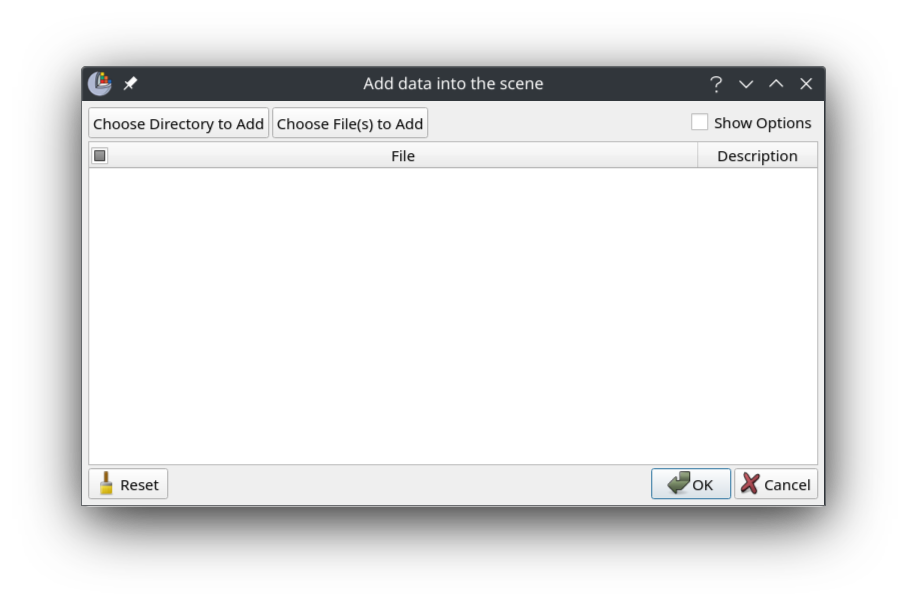
\includegraphics[
			% scale=0.2
			width=0.90\paperwidth
		]{filepicker.png}}
	\caption{3D Slicer file picker}
	\label{fig:filepicker}
  \end{figure}
  \begin{figure}[h!]
	\centerline{
		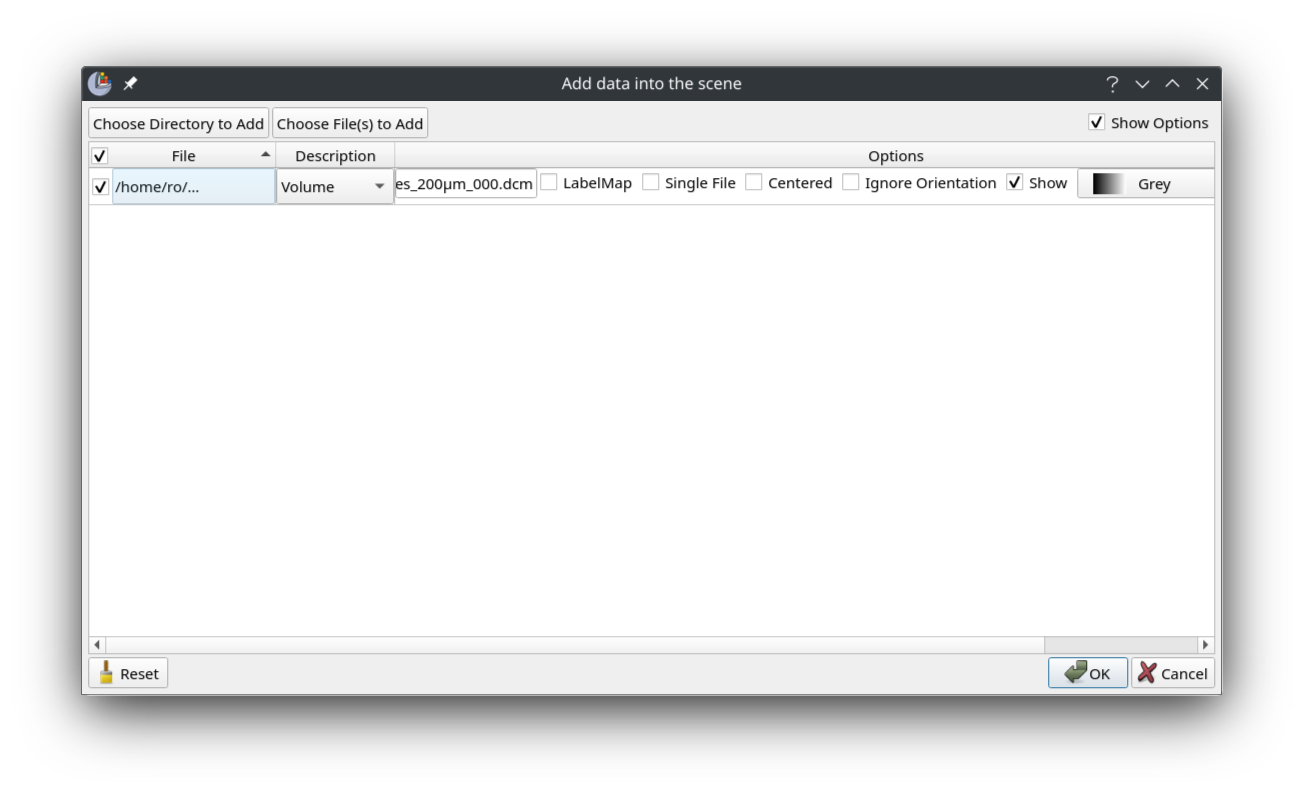
\includegraphics[
			% scale=0.2
			width=0.90\paperwidth
		]{filepicker2.png}}
	\caption{3D Slicer file picker options}
	\label{fig:filepicker2}
\end{figure}
\noindent
Depending on whether the data is contained in a single or multiple files, click either \texttt{Choose Directory to Add} or \texttt{Choose File(s) to Add}. Browse to your data, select it and confirm your selection by clicking \texttt{Choose}.
Show additional import options by setting a checkmark at \texttt{Show Options}.
Here it is possible to load the dataset as a Label map, force 3D Slicer to ignore similar files, automatically center the volume, ignore orientation information in the DICOM header, show or hide the volume and set the color table.
After confirming the import, depending on size of the dataset, some patience may be required. If the import was successful and the dataset has not been set to be hidden after import, 3D Slicer will automatically populate the view area.

\subsection{Saving Data}
  \begin{figure}[h!]
	\centerline{
		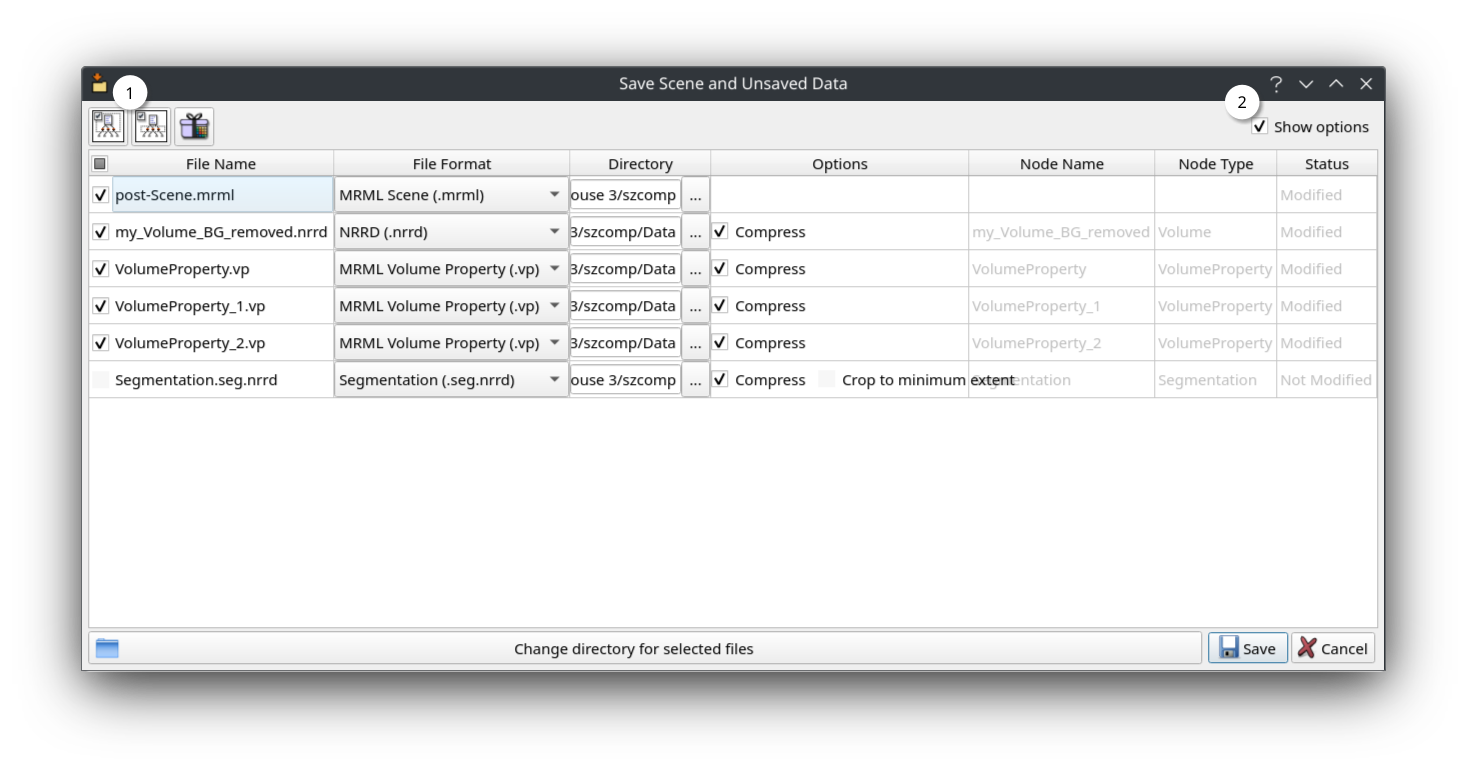
\includegraphics[
			% scale=0.2
			width=0.90\paperwidth
		]{saveMenu.png}}
	\caption{3D Slicer file save menu}
	\label{fig:save}
\end{figure}
Save your work in 3D Slicer by clicking on the \texttt{Save Data} button in the \cref{fig:toolbar}:3.
This will open a popup window which holds information about what data will be saved and the format it will be saved to.
3D Slicer defaults to bundling up your data into a single file. Change this by clicking on the bundle icon (\cref{fig:save}:1) and set a checkmark at \texttt{Show options} (\cref{fig:save}:2).
The window should now look like \Cref{fig:save}.
The first collumn shows the file names, which are derived from their names in the \texttt{Data} module and their file format.

Lets take a look at what 3D Slicer is going to save:

\begin{description}
\item [post-Scene.mrml] \textquote{MRML file is a xml-formatted text file with scene metadata and pointers to externally stored data files}\cite{kikinis3DSlicerPlatform2014} (Metadata file)
\item [my\_Volume\_BG\_removed.nrrd] volume data in a non-DICOM general purpose multi-dimensional format
\item [VolumeProperty.vp] volume property file storing information on volume rendering (Metatdata file)
\item [Segmentation.seg.nrrd] \textquote{Segmentation labelmap representation}\cite{kikinis3DSlicerPlatform2014} storing the segmentation as a multi dimensional volume
\end{description}

3D Slicer defaults to compressing all data before saving and there should be no reason to turn this behavior off.


The second column is dedicated to the file format of mentioned files.
3D Slicer supports a number of different file formats (see: \url{https://slicer.readthedocs.io/en/latest/user_guide/data_loading_and_saving.html#supported-data-formats}).
However, exporting for example a volume or segmentation in a different format, say STL for 3D printing, I recommend choosing the \texttt{Data} module over changing file formats in the save dialogue.
Compression can be turned off or on per file in the options column.
And somewhat importantly, the last column, the status column, shows if a file has been modified since the last save.

Clicking on the ``Bundle'' icon (\Cref{fig:save}:1) collapses the file view, as this instructs 3D Slicer to not save individual files, but bundle them in a \Gls{mrb} file.

\pagebreak

\subsection{Addressing Performance issues}
If loading the data took a long time or scrolling in the 2D views is sluggish, %TODO: insert subsection about memory usage and performance
it might be worth considering reducing the size of your dataset.
Make sure to save after every operation to reduce the loss of progress in case of a crash.

\subsubsection{Cropping} \label{crop}
Locate the \texttt{Crop Volume} module either via the dropdown menu
% TODO: insert reference to image
\texttt{Converters -> Crop Volume} and switch to it.
\begin{figure}[h!]
	\centerline{
		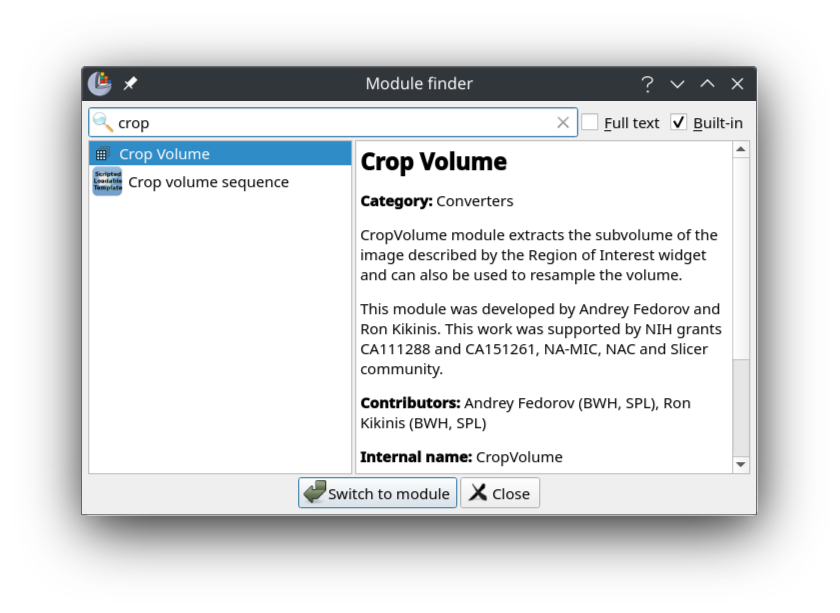
\includegraphics[
			% scale=0.2
			width=0.90\paperwidth
		]{moduleSwitcher.png}}
	  \caption{3D Slicer module switcher}
	  \label{fig:mS}
\end{figure}
Or click the lens icon to use the text search (see: \cref{fig:mS})
Before any cropping can happen it is required to do some setup in the newly opened module panel.
\begin{figure}[h!]
	\centerline{
		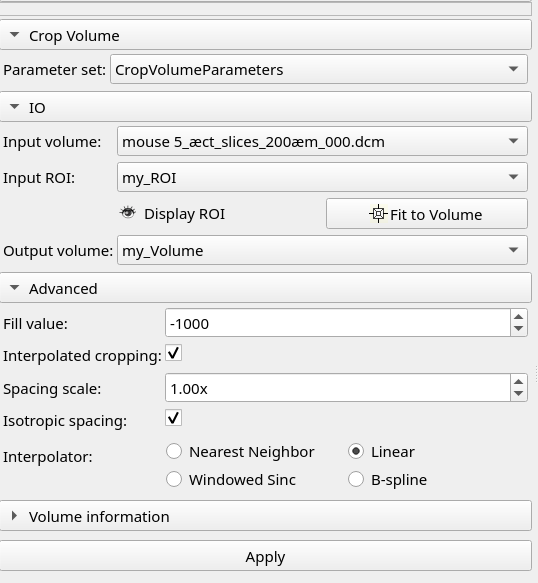
\includegraphics[
			scale=0.8
			%width=0.90\paperwidth
		]{croppingModulePanel.png}}
	  \caption{3D Slicer cropping module panel}
	  \label{fig:cMP}
\end{figure}
See \cref{fig:cMP} for reference.
Under \texttt{IO -> Input Volume} make sure the dataset you loaded is selected.
Create a new ROI under \texttt{IO -> Input ROI} choose \texttt{Create new ROI as...} and give it a distinctive name. Also make sure it is not hidden by looking for an open eye next to \texttt{Display ROI}.
Next choose a name for your output volume under \texttt{IO -> Output volume -> Create new volume as...} and give it a distinctive name.
Under \texttt{Advanced -> Fill value} choose a HU value for everything outside your ROI. It should be easily distinguishable from the structure or tissue you are segmenting. For bone segmentation I recommend choosing -1000 HU\footnote{The HU value of air}. Checking the tickbox \texttt{Advanced -> Interpolated cropping} will ensure that the output volume has the same dimensions as the input volume.
%%TODO: detour about compression???
Also check the box: \texttt{Advanced -> Isotropic spacing} with a \texttt{Spacing scale} of 1x to ensure the voxels stay isotropic.
Now adjust your ROI in the 2D view areas by clicking and dragging the colored dots at the edges and corners of the ROI.
Crop out as much excess volume as possible without affecting the anatomy you wish to segment.
Check positioning and size of your ROI by scrolling through the 2D view on all three planes, after that click \texttt{Apply}.
This operation might require some patience depending on the size of the dataset.
Note that there will be no visual confirmation the cropping operation is finished.
However, you can check by switching to the \texttt{Data} module.
If 3D Slicer is unresponsive, the operation is not done yet.
\begin{figure}[h!]
	\centerline{
		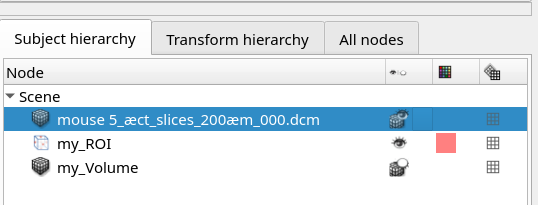
\includegraphics[
			scale=0.9
			%width=0.90\paperwidth
		]{cropConfirm.png}}
	  \caption{3D Slicer data module}
	  \label{fig:cC}
	\end{figure}
	\pagebreak
	\newline
Under \texttt{Subject hierarchy -> Node -> Scene} (see: \cref{fig:cC}) you should see:
\begin{enumerate}
  \item the loaded dataset
  \item the newly created ROI
  \item the newly created volume
\end{enumerate}
Show your cropped volume by clicking on the closed eye on the same line as its name. Hide the ROI by clicking on the open eye next to its name.
3D slicer will then automatically hide the original dataset and populate the view area with the cropped volume dataset.

\subsubsection{Masking}\label{mask}
In the last step we cropped out the part of the source volume which does not contain any material/tissue of interest.
This step is dedicate to homogenizing the volume which was not cropped out in the last step.
\begin{figure}[h!]
	\centerline{
		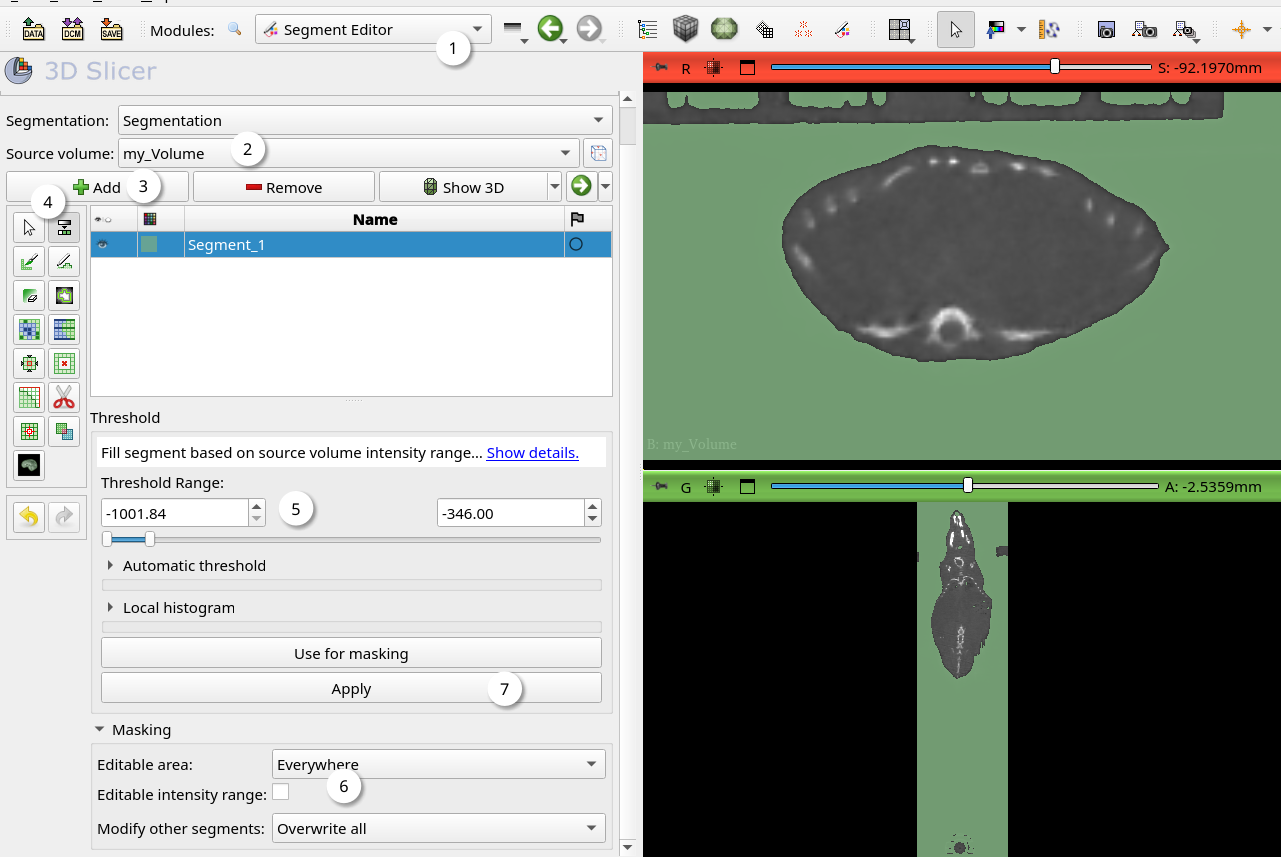
\includegraphics[
			%scale=0.5
			width=1.3\textwidth
		]{thesholdMasking.png}}
	  \caption{Threshold background}
	  \label{fig:tM}
\end{figure}
Switch to the \texttt{Segment Editor} module (see: \cref{fig:tM}:1).
Make sure your cropped volume is selected as the \texttt{Source volume} (see: \cref{fig:tM}:2).
Click on the \texttt{+ Add} button (\cref{fig:tM}:3). You should see a new segment appear in the segments list below.
Double click to rename it to ``Background'' or leave its default name.
Make sure your ``Background''segment is select and then activate the \texttt{Threshold} tool (\cref{fig:tM}:4).
Shift the lower threshold limit until the background is covered by the segment color in the 2D views. Afterwards shift the upper threshold limit until your tissue of interest is definitely no longer covered by the segment color.
Before applying (\cref{fig:tM}:7) the threshold segmentation make sure that 3D Slicer is allowed to edit \texttt{Everywhere} and overwrite all other segments (see: \cref{fig:tM}:6).

\pagebreak
\begin{figure}[h!]
	\centerline{
		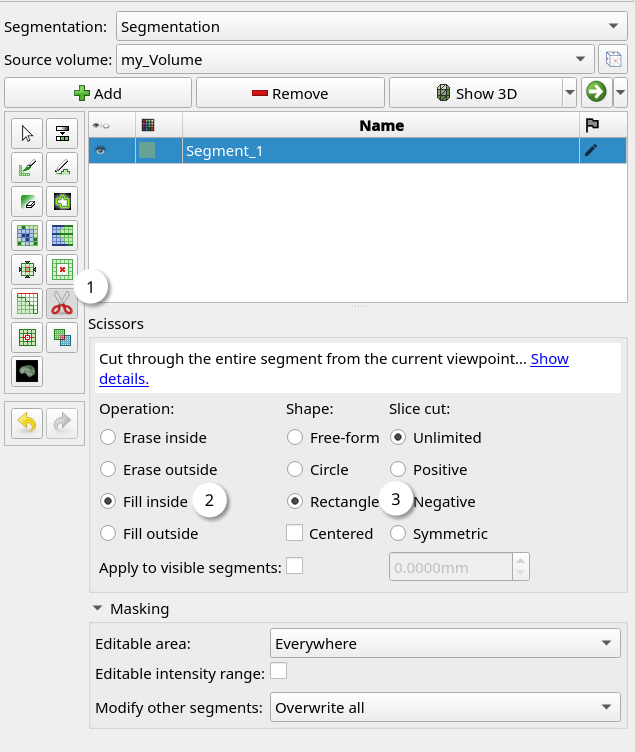
\includegraphics[
			scale=0.8
			%width=0.80\paperwidth
		]{scissorsMasking.png}}
	  \caption{Scissors background}
	  \label{fig:sM}
	\end{figure}
\noindent
Next, activate the \texttt{Scissors} tool (see: \cref{fig:sM}:1) with your ``Background'' segment selected.
This tool provides a simple way of selecting materials and tissue that are not easily distinguished by HU value, like the MicroCT couch and positioning tools.
Change its operation mode to \texttt{Fill inside} (\cref{fig:sM}:2) and its shape to \texttt{Rectangle} or \texttt{Free-form} (\cref{fig:sM}:3).
In the 2D views you can now click and drag to create a shape, upon releasing the left mouse button the tool will add the volume inside the shape to your ``Background'' segment.
\newline % sample hint
\newline
\begin{minipage}{0.4\textwidth}
  \begin{center}
	\includesvg[
		inkscapelatex=false,
		width = 0.6\textwidth
	]{hint.svg}
\end{center}
\end{minipage}%
%
\begin{minipage}{0.5\textwidth}
    The scissors tool ``punches'' through the volume, this makes it very easy to accidentally select something intentionally. Always make sure there is no ROI in the area on the previous or next slices and check your positioning on the other planes. In most cases it will be easier to work on small sections of your volume, rather than selecting a large volume in one single step.
\end{minipage}
\newline
\newline % sample hint

\pagebreak
\begin{figure}[h!]
	\centerline{
		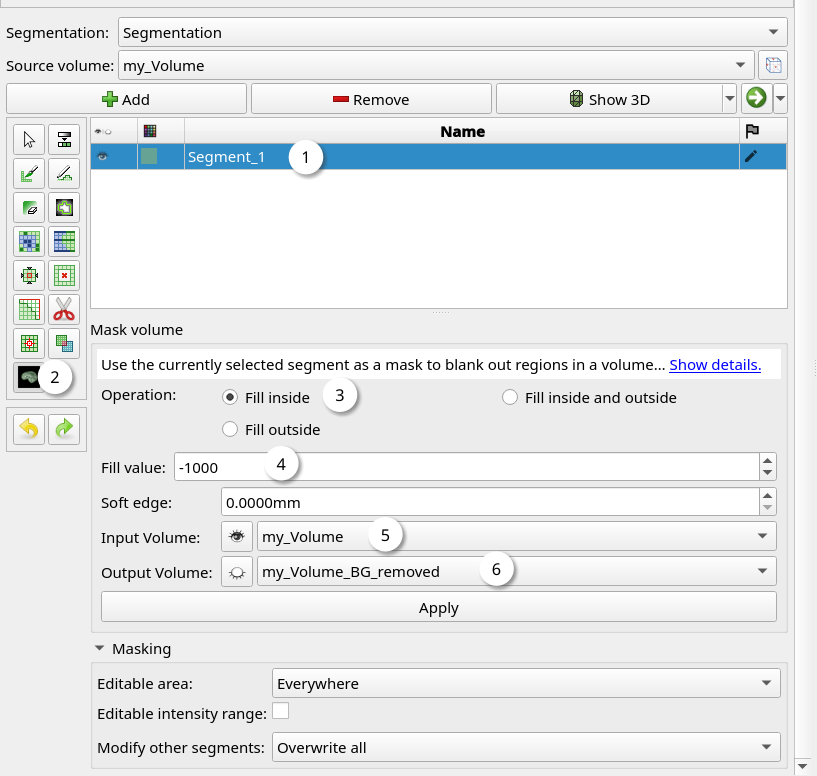
\includegraphics[
			%scale=0.8
			width=1.2\textwidth
		]{maskBG.png}}
	  \caption{Mask background}
	  \label{fig:mBG}
	\end{figure}
\noindent
Activate the \texttt{Mask volume} tool (see: \cref{fig:mBG}:2) and make sure your ``Background'' segment is selected (\cref{fig:mBG}:1).
As for the operation mode, choose \texttt{Fill inside} (\cref{fig:mBG}:3).
The fill value (\cref{fig:mBG}:4) should be the same as in the cropping step (\cref{crop}).
Select your cropped source volume as the \texttt{Input Volume} (\cref{fig:mBG}:5).
For the result, create a new volume by clicking on \texttt{Output Volume -> Create new Volume as...} (\cref{fig:mBG}:6) and give it a distinctive name.
\newline % sample hint
\newline
\begin{minipage}{0.4\textwidth}
  \begin{center}
	\includesvg[
		inkscapelatex=false,
		width = 0.6\textwidth
	]{irreversible.svg}
\end{center}
\end{minipage}%
%
\begin{minipage}{0.5\textwidth}
  Always create a new volume when working with the \texttt{Mask volume} tool.
  It overrides the individual voxel intensity values, this \emph{can not be undone} as 3D Slicer does not store the original intensity values in its undo history.
\end{minipage}
\newline
\newline % sample hint
\pagebreak

\subsubsection{Cleanup}
Switch to the \texttt{Data} module.
\begin{figure}[h!]
	\centerline{
		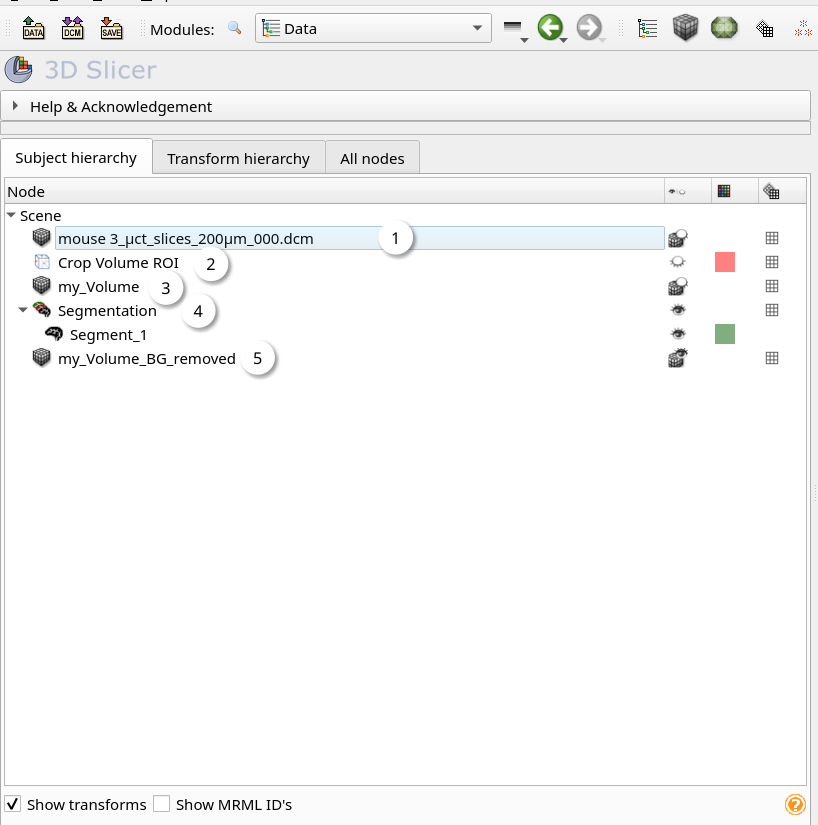
\includegraphics[
			%scale=0.8
			width=1.2\textwidth
		]{cleanup.png}}
	  \caption{Data cleanup}
	  \label{fig:clr}
	\end{figure}
\noindent
Here we see all the items we have created so far.
\Cref{fig:clr}:1 is the dicom dataset from the MicroCT scanner.
\Cref{fig:clr}:2 is the cropping ROI created in \cref{crop} and \cref{fig:clr}:3 is the volume that resulted from the cropping operation.
The segmentation item (\cref{fig:clr}:4) holds all segmentations created in the \texttt{Segment Editor} module. So far it only holds the ``Background'' segment created in \Cref{mask}. And the final item (\cref{fig:clr}:5) is the most recent volume resulting from the \texttt{Mask volume} operation.
Items \cref{fig:clr}:1-4 can be deleted to save Harddrive space and RAM while working in 3D Slicer.
\noindent
In this example the data volume on disk could be decreased from 309 megabytes to (source dicom data) to 15 megabytes.
Which equates to approximately a 95\% reduction in file size.
As a result of this, 3D Slicers RAM consumption has dropped from 1.3 gigabytes to 585 megabytes, which equates to approximately 55\% reduction.
See \Cref{measuements:memComp} for more information.
\begin{figure}
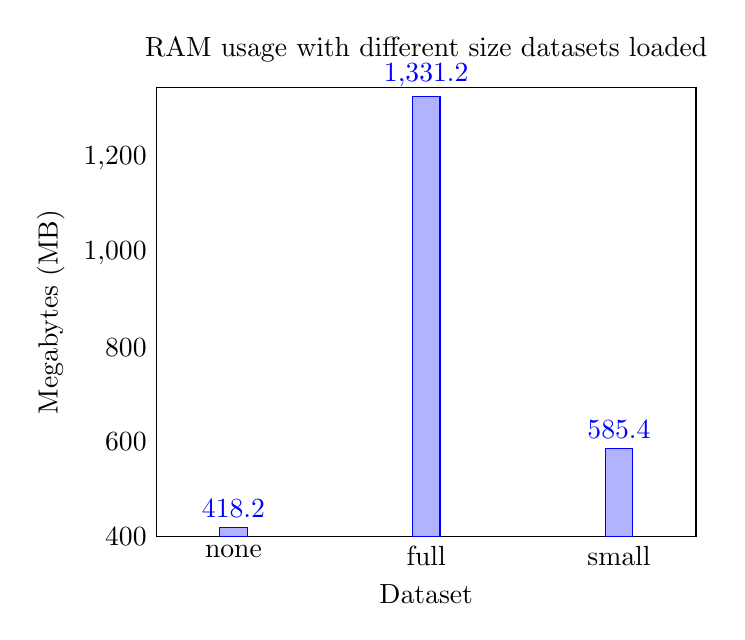
\begin{tikzpicture}
  \begin{axis}[
		title = RAM usage with different size datasets loaded,
		ybar,
		tickwidth = 0pt,
		xtick = data,
		enlarge y limits = 0.02,
		enlarge x limits = 0.2,
		ylabel={Megabytes (MB)},
		xlabel={Dataset},
		symbolic x coords = {none, full, small},
		nodes near coords
		]
    \addplot+ coordinates {
			(none, 418.2)
			(full, 1331.2)
			(small, 585.4)};
  \end{axis}
\end{tikzpicture}
\caption{RAM usage comparison}\label{fig:ramUC}
\end{figure}
\pagebreak


\section{Methode}
\begin{figure}[h!] % h - here
	\centerline{
		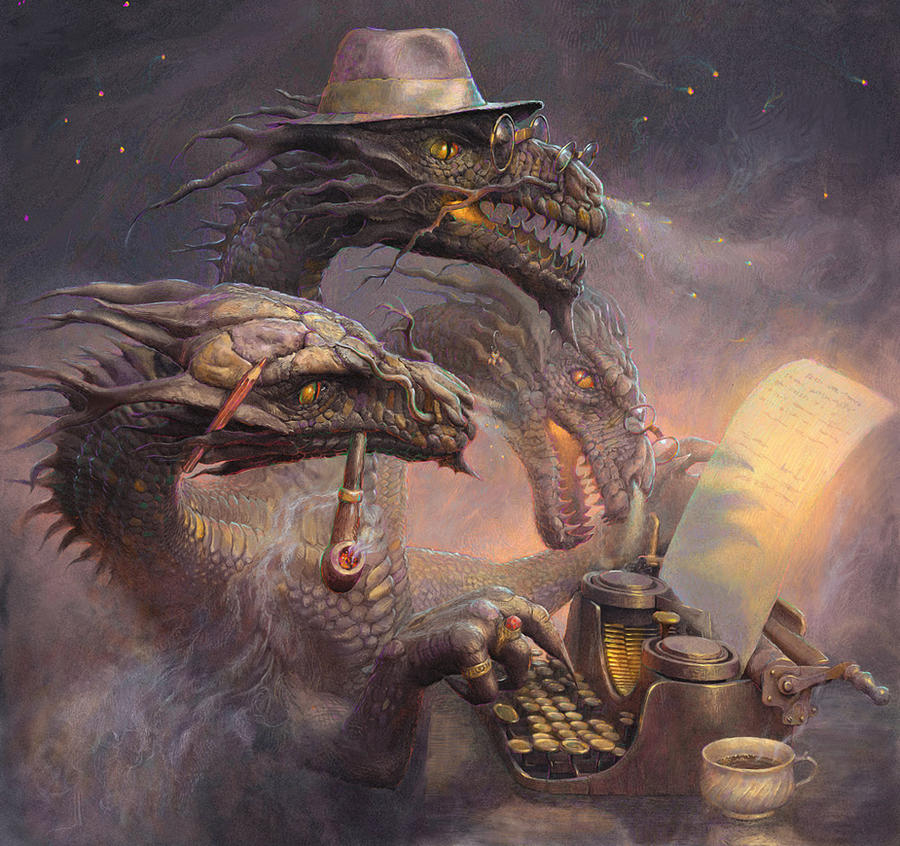
\includegraphics[
			% scale=0.2
			width=0.95\paperwidth
		]{../images/dragon.jpg}}
	\caption{Here be dragons}
	\label{fig:slicerWelcome}
\end{figure}
